\section{Single-source management in precision medicine}

In the fast-evolving field of precision medicine, managing documentation, data, and software development requires a robust approach to maintain consistency and accuracy across various studies, clinical trials, and software platforms. Our group adopts a \textbf{single-source management} philosophy, centralising shared components to reduce redundancy and prevent discrepancies.
This idea fit's with the "Everything as code" philosophy.


\subsection{Principles of single-source management}

Single-source management is predicated on the idea that all derivative documents and systems should draw from a common repository of information, ensuring that changes in one area are automatically propagated to all related areas. This approach is particularly advantageous in environments where:
\begin{itemize}
    \item Documentation needs to be consistent across multiple reports and publications.
    \item Software developments are closely tied to ongoing clinical trials and studies.
    \item Data from these trials and studies are frequently updated and must remain synchronised across platforms.
\end{itemize}


\textbf{Figure \ref{fig:precision_med_single_source_management}} illustrates why this is important. 
If a user requires a piece of critical information (for example, the number of patients in a study), it must be checked and copied. 
If that information later updates then all of the manual steps to find that information must also be repeated. 
When scaled across multiple different projects/uses, it rapidly degrades productive time into ``busy work'' for the user as well as leading to numerous critical errors.   
\textbf{Figure \ref{fig:precision_med_single_source_management}} illustrates why this is important. 
This illustration shows a two simple examples of where single-source management is used for two and six use cases, respectively. 

If, for example, the contents of ``raw data'' is updated as a project updates, all of the subsequent uses of this information can be automatically updated in a single step rather than repeating work numerous times. 
\textbf{!! N.B. } - Every edge which connects two nodes represents a task which must be performed; either manually or automatically using single-source management. 

\begin{figure}[h] \hspace*{0cm} 
\begin{center}
	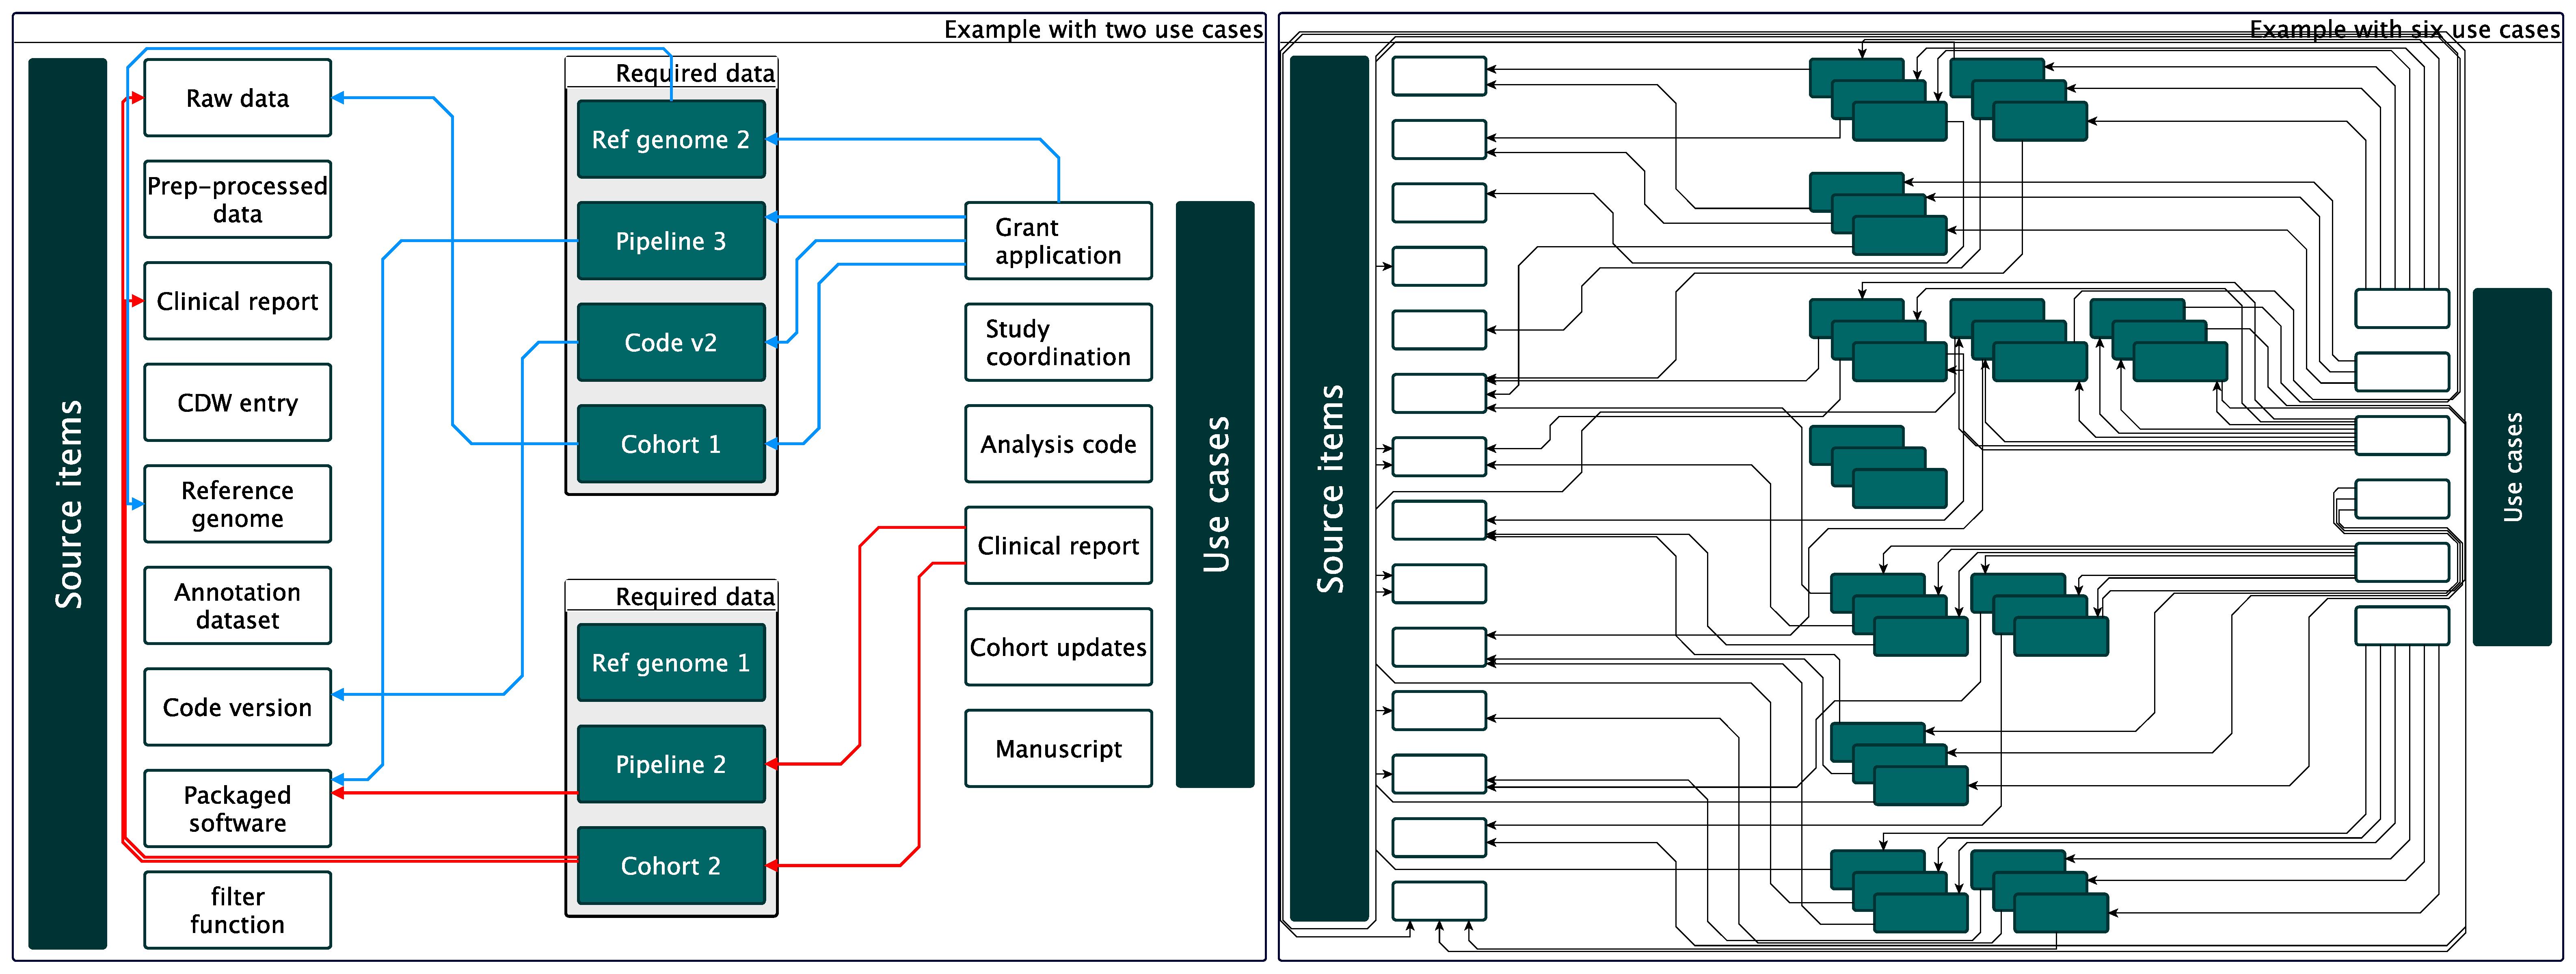
\includegraphics[width=1\textwidth]{precision_med_single_source_management}
	\caption{Single-source management examples within the \pmu. As the number of uses for information increases, the scale of tracking grows massively.  Every edge which connects two nodes represents a task which must be performed. Without automation, manually performing each task causes a bottleneck that can halt progress. 
	Single-source management allows us to update every edge automatically.}
	\label{fig:precision_med_single_source_management}
\end{center}
\end{figure}



\subsection{Implementation example in our documentation}

Our LaTeX documents exemplify this single-source management system. 
The document that you are reading has been generated using this system. 
For example, all of the \variablesdarkgreen{highlighted key texts} used in this document are sourced from a central repository so that they are always up-to-date.
Key elements such as common variables, formatting settings, and version-controlled content are centralised. 
We maintain a structured directory layout for efficient resource management:

\begin{verbatim}
/resources
    /head.tex            % Standardized layout and color definitions
    /variables           % Common variables across projects
        /variables.tex   % Definitions of constants, pipeline names, etc.
/main_document_1.tex    % Specific document drawing from the resources
/main_document_2.tex    % Another document sharing the same resources
\end{verbatim}

The same approach is taken in our software development, analysis protocols, data-flow, etc. 
There is no philosophical separation between any type of information - 
a document name is treated with the same respect as raw data from a patient.
There is a single source of truth for information and all subsequent uses of that information directly source the origin, ideally including tracked changes. 
Numerous sources of variables can be used, including the database repository, 
document layouts, 
and other configurations. 
The variables source contains declarations for key terms and concepts used across various documents, highlighted using a specific color to indicate their importance and frequent usage.
These variables serve not only as identifiers within texts/code/etc. but also help to  connect the reader/user with recurring themes and important concepts across multiple documents. 


\subsection{Example}
Long-term projects use data from a range of sources. 
Common databases or core files are often reused multiple times. 
Some data can remain dormant for long periods of time. 
In the following example from
\url{https://lawlessgenomics.com/data_usage_network},
we built automated data tracing systems that are used to present summarised analytics that are conducive to multipurpose usage and error prevention. 
This software scans entire data servers or project code to find and quantify all data sources. 
It then produces live interactive reports without the need for manual curation as shown in 
\textbf{figure \ref{fig:network_usage_plot_1}}.

\begin{figure}[h] \hspace*{0cm} 
\begin{center}
	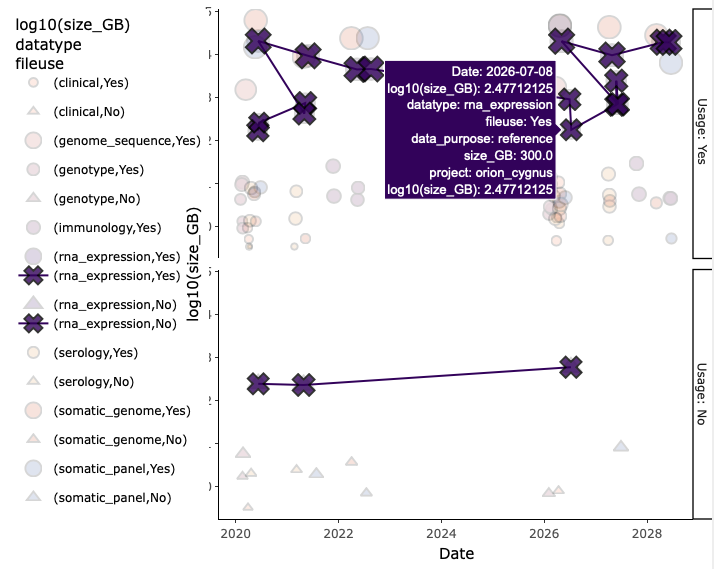
\includegraphics[width=.45\textwidth]{network_usage_plot_1}
	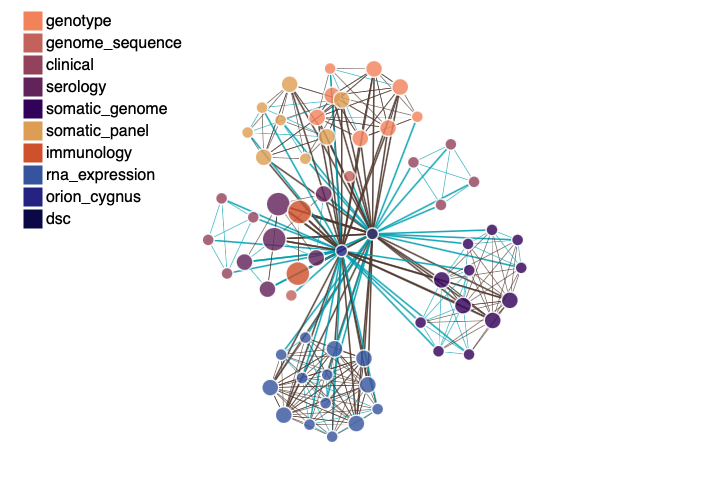
\includegraphics[width=.45\textwidth]{network_usage_plot_2}
	\caption{Left: Usage of all data showing dates, sizes, the purpose of usage, and projects. Double clicking a file will show all files that have the same datatype purpose (e.g. all files required for RNAseq analysis). Right: The interaction between data uses, within and between projects. Teal coloured edges illustrate single-purpose data. Dark coloured edges illustrate multi-purpose data.
}
	\label{fig:network_usage_plot_1}
\end{center}
\end{figure}

\subsection{Benefits}

The benefits of single-source management in our precision medicine research are manifold:
\begin{itemize}
    \item \textbf{Increased efficiency}: Updates need only be made in one place, automatically propagating to all documents and systems.
    \item \textbf{Enhanced accuracy}: Reduces the risk of discrepancies between documents, as all draw from a unified source.
    \item \textbf{Improved collaboration}: Team members can work simultaneously on different documents, confident that they are using the most current and consistent information.
\end{itemize}

Implementing this system requires rigorous discipline and a well-organised file management structure, but the return on investment in terms of time saved and error reduction is substantial.

